% Chapter 1

\chapter{Introduction} % Main chapter title

\label{Chapter1} % For referencing the chapter elsewhere, use \ref{Chapter1} 

\lhead{Chapter 1. \emph{Introduction}} % This is for the header on each page - perhaps a shortened title

%----------------------------------------------------------------------------------------

\section{Multimodal Representation Learning}
What is \ac{MRL} and why is it useful? These are the questions that I will address in this thesis.
Briefly, \ac{MRL} is the act of learning an abstract representation of sensory data from multiple sensors. As sensors respond directly to the world in which they are situated, \ac{MRL} is closely related to learning a world representation. Therefore, an accurate representation of sensory data contains in it, a representation of the world.

\ac{MRL} is therefore useful any time we have more than one sensor and if we can abstract sensory data to learn more about the world, or how the different modalities relate to one another. Perhaps the best example of this is Language Learning - when a baby learns its first words, it is doing \ac{MRL}, learning the association of sounds to objects and actions and vice-versa.

Beyond the highly complex and abstract task of learning a language, \ac{MRL} can also be used for sensor fusion. Providing auxilory information using extra sensors can help to improve classification accuracy (which I will demonstrate in \autoref{Chapter4}) and can also be used to regenerate missing data when only one modality is available.  A good example of this is when humans read lips in noisy environments, using the shape of the mouth to help recognise which words are being uttered even if they are not heard.


\section{Motivation}
One of the major challenges in robotics and machine learning is that of knowing how to develop systems capable of life long learning. If robots are to become common place in society, they must be capable of continuing to learn throughout their lives. They will not be very useful if they cannot learn new things that they were not programmed with at the factory.

\ac{MRL} addresses this by providing an unsupervised method for extracting useful and actionable information about the world. Let us return to the language learning scenario, except this time, instead of a baby, lets imagine a robot, fresh out of the box. Whilst we might expect that a robot would have some proficiency with language built into it, we cannot expect it to know the meaning of every single word, especially given the flexible and evolving way that humans use language. Our robot therefore needs a way to learn the meaning of new words - otherwise known as symbol grounding. 

Similarly, we cannot expect the robot to be able to recognise every single object in its environment. On my desk I have a Stirling engine, I would wager that most people who read this do not know what a Stirling engine is. However, if I showed you a picture of a Stirling engine (like the one in \autoref{fig:stirling}) you would be able to recognise what a Stirling engine is in future. Ideally, robots need to be able to do this.

\begin{figure}
\centering
	\includegraphics[width=0.3\textwidth]{Figs/introduction/stirling.jpg}
	\caption{The Stirling engine from my desk.}
	\label{fig:stirling}
\end{figure}

\begin{figure}
\centering
\begin{tikzpicture}
[node distance=1.5cm,
    every node/.style={fill=white, font=\sffamily}, align=center]
  % Specification of nodes (position, etc.)
  \node (object)   [activityStarts]              					{Object};
  \node (name)     [activityStarts, right of=object, xshift=4cm] {Name};
  
  \node (A)        [activityStarts, below of=object, yshift=-0.7cm]          {\includegraphics[width=0.96cm,height=1.5cm]{Figs/introduction/stirling.png}};
 \node (stirling) [activityStarts, right of=A, xshift=4cm]  {``Stirling Engine"};       
 
  % Specification of lines between nodes specified above
  % with aditional nodes for description 
  \draw[<->]     (object) -- (name);
  \draw[<->]     (A) -- (stirling);
 
\end{tikzpicture}
\caption{The bi-directional nature of language learning.}
\label{fig:bi_ll}
\end{figure}

The Stirling engine example shows how language learning is a bi-directional process. Not only do you need to learn the name of the object \textit{Stirling Engine} but also that the words \textsc{Stirling Engine} mean the object \textit{Stirling Engine} as shown in \autoref{fig:bi_ll}. 

Multimodal representation learning allows us to jointly model both the object \textit{Stirling Engine} and the words \textsc{Stirling Engine}, relying on only one assumption: \textbf{Sensory percepts which occur together are related}.

Whilst this may not be true for all sensory percepts it is true enough that co-occurrence of percepts allows us to infer useful information about the relationship between different modalities. For example, Smith et al. \cite{smith2008infants} show how infants learn object names based on ``cross-situational statistics'' i.e. how often a word and an object occur together. \autoref{fig:cross_sitch} illustrates this idea.

\begin{figure}[h]
\centering
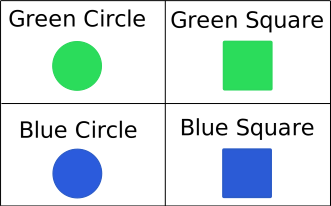
\includegraphics[width=0.5\textwidth]{Figs/introduction/shapes.png}
\caption{Associations among words and objects across multiple ambiguous scenes allow learners to find the proper mapping of words:
\textsc{Circle}, \textsc{Square}, \textsc{Green} and \textsc{Blue} to the shapes and colours: \textit{Circle},  \textit{Square},  \textit{Green} and \textit{Blue}}
\label{fig:cross_sitch}
\end{figure}

Looking at \autoref{fig:cross_sitch}, we can see that from a single example, it is not possible to disambiguate which word refers to which part of the image, i.e. we cannot ground the words \text{Green Circle} to the visual percepts \textit{Green} and \textit{Circle}. However, given two examples, it is very easy for an adult human to disambiguate what each word means. As we are given more examples, we can be more and more certain about what we believe the meanings of the words are. 

In the real world, visual perception is much noiser than the images presented in \autoref{fig:cross_sitch} as are the utterances of words. However, by providing more examples, we can overcome the challenges presented by this as shown in \cite{yurovsky2013statistical}. In this thesis I will show how \ac{MRL} can be applied to this problem and solve it, learning the meanings of different word types, such as object names, colours, sizes and positions as well as the inverse problem, generating these labellings for images of objects. \autoref{fig:mrl_teaser} shows a few examples of \ac{MRL} solving this problem.

\begin{figure}
\centering

\includegraphics[width=0.75\textwidth]{Figs/chapter6/avgBrickDuckBGYGeneratedExemplars.png}
\caption{Images generated from textual descriptions (B, M and S are Big, Medium and Small, respectively) by the system developed in this thesis.}
\label{fig:mrl_teaser}
\end{figure}

\section{Hypotheses}


\begin{enumerate}

	\item \textcolor{red}{\ac{MRL} can be used to learn the association between sounds and the visual symbols they represent. I.e. to solve the symbol grounding problem.}
	\item \textcolor{red}{\ac{MRL} enhances classification accuracy of sounds and visual symbols.}
	\item \textcolor{red}{\ac{MRL} can be used to learn language as it relates to the visual properties of objects. I.e. to solve the symbol grounding problem.}
	\item \textcolor{red}{\ac{MRL} can be improved through transfer learning.}
	\item \textcolor{red}{The multimodal representation learnt by the \acp{MAE} exhibits all of the desirable properties of a representation as layed out by Bengio et al. in \cite{repRev}.}		
	\item \textcolor{red}{It is possible to use \ac{MRL} with real data.}
	
\end{enumerate}

\textcolor{red}{Hypotheses 1 and 2 are addressed in \autoref{Chapter4}, hypotheses 3, 4 and 5 are addressed in \autoref{Chapter5} and hypothesis 6 is addressed in \autoref{Chapter6}.} 


\section{Methodology}
\textcolor{red}{Throughout this thesis, the experiments are performed using a deep neural network architecture known as a \acl{MAE}. This architecture was chosen for its autoencoding nature, meaning that it is possible to train the system without human intervention, i.e. through unsupervised learning.} 

\textcolor{red}{The \ac{MAE} was used without a variational cost (as in a \acp{VAE}) as we cannot gaurantee that the latent space of the network should follow a particular distribution, which a variational cost would enforce.}

\textcolor{red}{Finally, the use of \acp{ANN} over other machine learning techniques is due to their flexible nature, requiring little to no feature engineering of the data used by the system. Further to this, \acp{ANN} have been shown to acheieve state-of-the-art results on many robotics, computer vision and natural language tasks.}

\begin{figure}
\centering
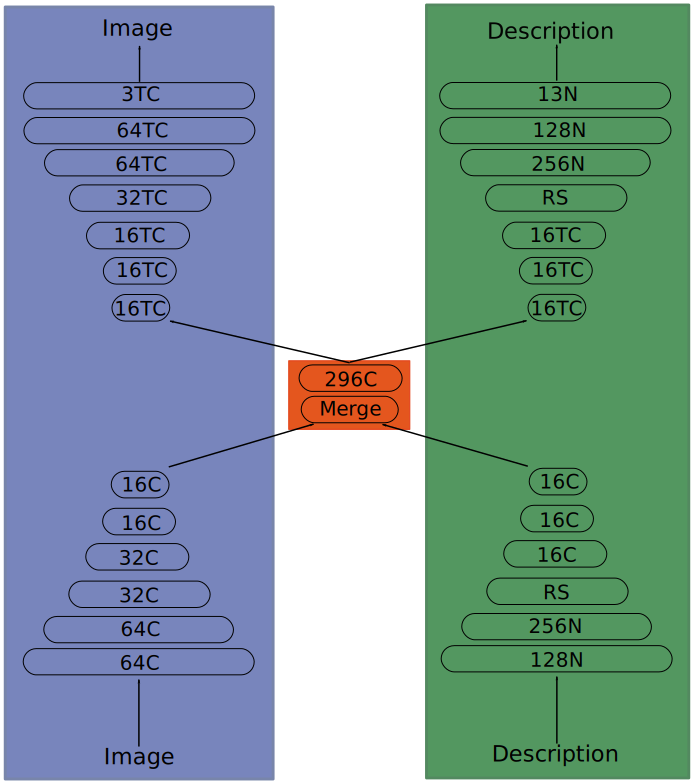
\includegraphics[width=0.75\textwidth]{Figs/shapes/maeArch.png}
\label{fig:final_arch}
\caption{\textcolor{red}{The architecture of the MAE used in \autoref{Chapter6} to generate the images seen in \autoref{fig:mrl_teaser}. Layers marked with C are convolution TC, Transposed Convolution, RS, Reshape and N, Dense.}}
\end{figure}

\textcolor{red}{\autoref{fig:final_arch} shows an overview of the \ac{MAE} architecture used in \autoref{Chapter6}. The \ac{MAE} used in \autoref{Chapter4} and \autoref{Chapter5} follow a very similar structure and are pictured later in \autoref{fig:netMnist} and \autoref{fig:netArts}.} 





%----------------------------------------------------------------------------------------






